\section{Theoretical part}

\subsection{The Internet Protocol}
\subsubsection{Addresses and network masks}
\begin{description}
    \item[Part 1.1:] From a router's point of view the purpose of network masks is to
        reduce the size of the forwarding table. Because all IP addresses in the same network
        have the same prefix, a router only needs to store the prefix.
    \item[Part 1.2:] Network masks may be expressed in the same dotted quad notation
        that IP addresses are expressed in (because they are also 4 bytes long).
        255.225.255.0 is not a valid network mask, because it is not a continuous
        prefix of 1-bits. In the slash-notation we would interpret /28 as a prefix
        of 28 1-bits, or the network mask 255.255.255.240.
    \item[Part 1.3:] The difference is that the network prefix was constrained to be of length
        8, 16 or 24 bits in classful addressing, and can be of any length in classless
        interdomain routing.
    \item[Part 1.4:] The network address is simply the IP anded with the network mask (byte form),
        and the broadcast address is the network address plus \\$2^{32-\text{prefixlength}} - 1$.
        The size of the network is $2^{\text{prefixlength}} - 2$ (subtracting 2 for the network
        and broadcast address). The available addresses are found in the interval between the network
        and broadcast address.

    %TODO: When I get a nice tool for it, very soon
    \item[Part 2.1:]
        Size of the network: 30\\
        Network address: 130.225.165.0\\
        Network mask: 255.255.255.224\\
        Broadcast address: 130.225.156.31\\
        First, fifth, last address: 130.225.165.1, 130.225.165.5, 130.225.165.30
    \item[Part 2.2:]
        Size of the network: 510\\
        Network address: 10.0.42.0\\
        Network mask: 255.255.254.0\\
        Broadcast address: 10.0.43.255\\
        First, fifth, last address: 10.0.42.1, 10.0.42.5, 10.0.43.254
    \item[Part 2.3:]
        %TODO: This is some strange shit
        Size of the network: 1\\
        Network address: 4.2.2.1\\
        Network mask: 255.255.255.255\\
        Broadcast address: 4.2.2.1\\
        First, fifth, last address: 4.2.2.1
    \item[Part 2.4:]
        Size of the network: 16382\\
        Network address: 192.38.64.0\\
        Network mask: 255.255.192.0\\
        Broadcast address: 192.38.127.255\\
        First, fifth, last address: 192.38.64.1, 192.38.64.5, 192.38.127.254
\end{description}

\subsubsection{Network Address Translation}
\begin{description}
    \item[Part 1:] NAT-enabled routers handle multiple connections by maintaining a NAT translation
        table that maps pairs of internal IPs and ports to external ports. Each connection is given
        an external port in the router, such that traffic going back to the router can be de-multiplexed
        and sent to the appropriate internal IP and port.
    \item[Part 2:] Because ports are limited to 16 bits, there are only 65536 possible ports to choose from.
        If 65536 long lived connections are opened by the internal hosts, no further mappings can be made in
        the NAT translation table. The routers ports are exhausted, and no further connections can be made.
    \item[Part 3:] NAT breaks the layering principle of the Internet because it alters the contents of the
        transport layer port field. This is not allowed in the layering model, because a router only handles
        the layers up to the network layer.
\end{description}

\subsection{Distributed Hash Tables}
\begin{description}
    \item[Part 1:] The routing table for node 1 is as follows\\
        \begin{tabular}{|c|c|c|}
            \hline
            $i$ & $id + 2^{i}$ & $succ$ \\ \hline
            0 & 2 & 3 \\ \hline
            1 & 3 & 3 \\ \hline
            2 & 5 & 6 \\
            \hline
        \end{tabular}

    \item[Part 2:] A query for item 5 (from node 1) will be received by node 6 directly.
    \item[Part 3:] A query for item 5 (from node 7) will be received by node 3 and 6.
\end{description}

\subsection{SSH Tunneling}
\subsubsection{{\sc Echoserver} $\leftrightarrow$ {\sc Client}}
\begin{description}
    \item[Question 1:] At this point the echo server is waiting for clients to connect to it. It is blocking on
        the accept call at line 24.
    \item[Question 2:] The port number appears in both established sockets because it is in the source of the client's
        socket, and the destination of the server's socket (TCP if full duplex, so there is a connection in both directions).
        The port number was chosen randomly as the port for the client's outgoing connection.
    \item[Question 3:] One can see all messages sent to and from the server in the TCP dump. This is because they are sent. See \autoref{sub:q3-tcp} for TCP dump.
        unencrypted over the network (so every hop on the way will also be able to read them).
    \item[Question 4:] No it's not possible to establish a connection. The connection is blocked by a firewall on ask.diku.dk % TODO: use nmap
    \item[Question 5:]  host = 'localhost', port = 6790. We can communicate this way, because the data sent to port 6790 on our localhost is forwarded to ask.diku.dk on port 6002 though our SSH tunnel.
    \item[Question 6:] One can again see the messages sent to and from the server in the TCP dump. The data is not encrypted when sent between SSH tunnel and the echoclient, only when going though the SSH tunnel. See \autoref{sub:q6-tcp} for TCP dump.

    \item[Question 7:] One can only see scrampled data by the TCP dump. This is caused by we are monitoring SSH traffic, which is encrypted. SSH runs on port 22. See \autoref{sub:q7-tcp} for TCP dump.

    \item[Question 8:]
    % client on local ( 52926 ) client SSH tunnel connection ( 52926 <=> 6790 ), magically transformed into 6002 on ask.diku.dk, where the TCP socket for this client has been created at port 35299. -- SSH connection ( 39676 <=> 22 )
    See \autoref{fig:ssh-q8}.
    \begin{center}
    \begin{figure}[H!]
        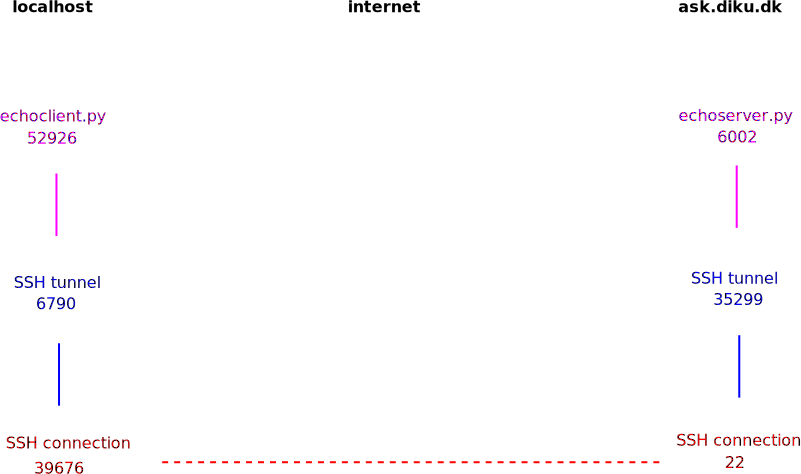
\includegraphics[width=0.5\paperwidth]{graphics/ssh-q8.pdf}
        \caption{\label{fig:ssh-q8}Overview of the connections. Dashes lines represents encrypted messages}
    \end{figure}
    \end{center}
\end{description}
